\subsection{Related Technologies}
It is almost always beneficial for developers of a product to research and study related or similar products, as well as products related to their product's subsystems, in detail to gain a better understanding of how a subsystem can operate, and how subsystems can integrate with each other to form a cohesive system. In this section, members of our team explore technologies and solutions related to our product and its various subsystems. Some of the technologies studied below can be, and most likely will be integrated into our final product.

\subsubsection{Ocean insight: Ocean ST NIR Microspectrometer}
Ocean Insight is a local manufacturer of high-end, low size, weight, and power spectrometers. The ST NIR Microspectrometer is about 40 cubic centimeters in volume with a scan speed of 10ms, a signal to noise ratio of 190:1, and a spectral resolution of 2.2nm. Its spectral range is from 645nm to 1085nm, and it was specifically designed to be integrated into larger systems for customers who were interested in a flexible, low-cost design. Added to that, the system is rugged, and offers a variable slit input size, increasing its flexibility even further. While the designs are proprietary, this system serves as a benchmark for what can be achieved by the industry, and no doubt there are major design changes that can be made to achieve a similar result for the application intended for the Auto Garden Bed. That being said, the selling price for one is \textdollar1,750.
\begin{figure}[H]
    \caption{Ocean ST NIR Microspectrometer}
    \centering
    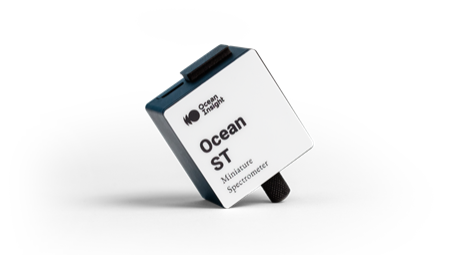
\includegraphics[width=0.5\textwidth]{images/3-2-1Pic.png}
\end{figure}
\subsubsection{AgroCares Nutrient Soil Scanner}

AgroCares offers a Near Infrared Spectrometer specifically designed for Proximity Soil Sensing. Its spectral range is from 1300 to 2500nm and it uses Micro Electrical Mechanical Systems or MEMS to capture EM Waves reflecting off the soil. The real value of the product is in its wireless communications system. The device uses Bluetooth 4.0 to send data to a cloud data center. There, spectrographs of large data sets of soil with known nutrient contents are compared with the reading, cutting out the need for on-sight calibration. The system is handheld and uses eight tungsten halogen bulbs to blast the soil with energy. This light is collected in an extremely small area, sampling 65 squared millimeters. It would be worth researching to see if the Tungsten bulbs were linked to the 1300 to 2500nm spectral range or if another probe and sensor would suffice.
\begin{figure}[H]
    \caption{AgroCares Nutrient Soil Scanner}
    \centering
    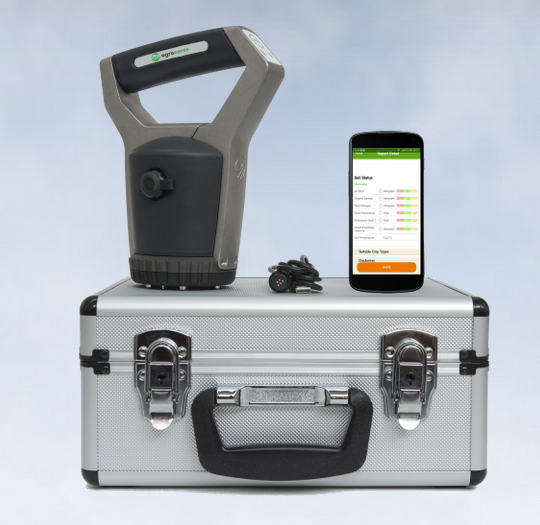
\includegraphics[width=0.5\textwidth]{images/3-2-2Pic.png}
\end{figure}

AgroCares offers a Near Infrared Spectrometer specifically designed for Proximity Soil Sensing. Its spectral range is from 1300 to 2500nm and it uses Micro Electrical Mechanical Systems or MEMS to capture EM Waves reflecting off the soil. The real value of the product is in its wireless communications system. The device uses Bluetooth 4.0 to send data to a cloud data center. There, spectrographs of large data sets of soil with known nutrient contents are compared with the reading, cutting out the need for on-sight calibration. The system is handheld and uses eight tungsten halogen bulbs to blast the soil with energy. This light is collected in an extremely small area, sampling 65 squared millimeters. It would be worth researching to see if the Tungsten bulbs were linked to the 1300 to 2500nm spectral range or if another probe and sensor would suffice.


\subsubsection{Web Technologies}\label{sec:web-tech}
\paragraph{Docker}
``Docker is a platform designed to help developers build, share, and run modern applications. We handle the tedious setup, so you can focus on the code.'' This quote comes directly from Docker's website on why developers should switch to Docker. This technology makes items more portable by making the executable platform agnostic through the use of a docker kernel and containers. The figure below should provide some clarity:

\begin{figure}[H]
    \caption{Docker architecture}
    \centering
    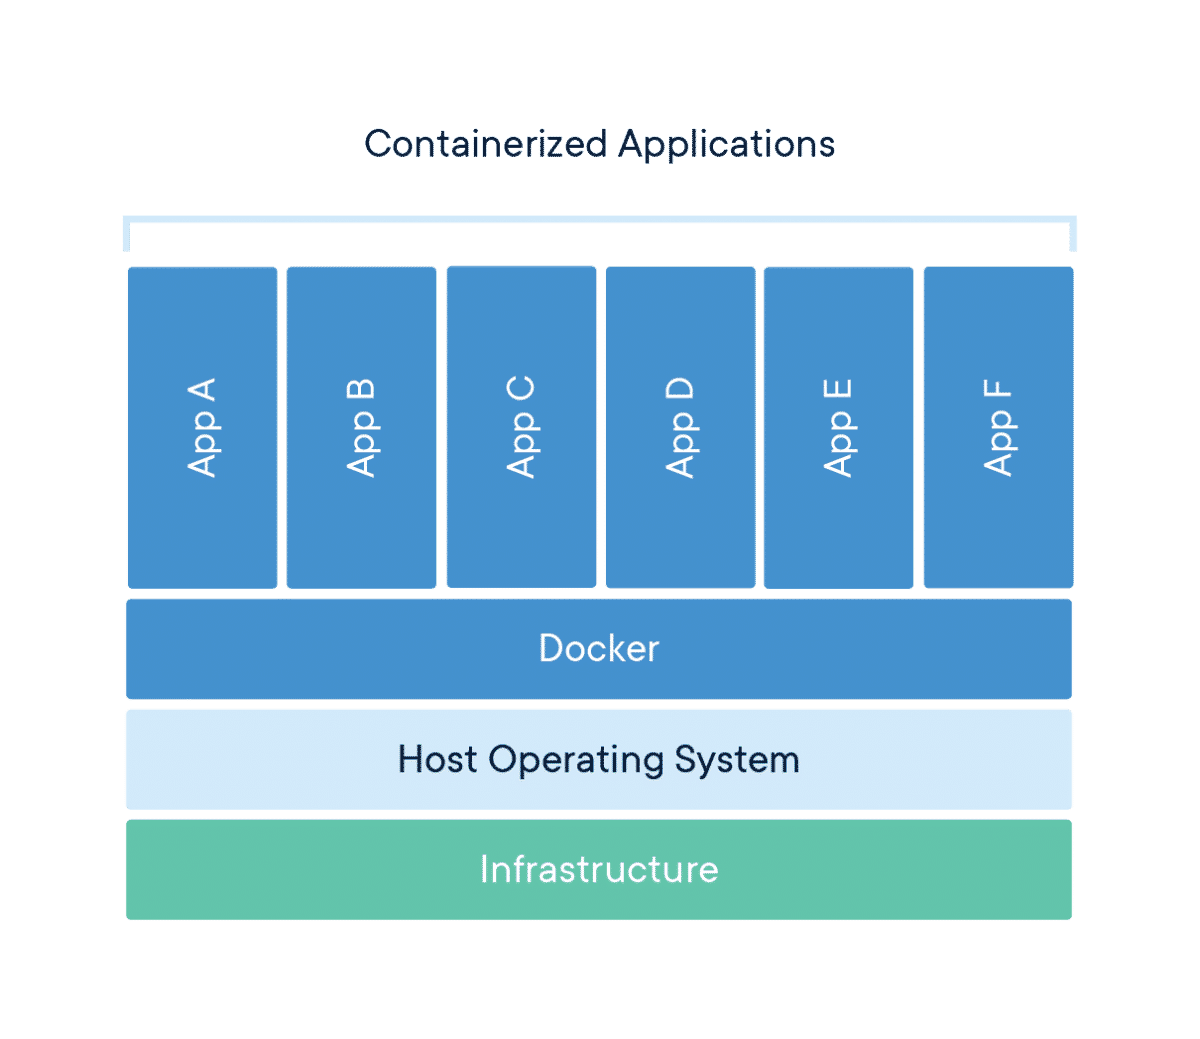
\includegraphics[width=\textwidth]{images/Docker-Architecture.png}
    \label{fig:docker_arch}
\end{figure}

A developer can program applications such as those demonstrated in figure \ref{fig:docker_arch}, package them into images and run them in containers. Docker works with the OS kernel to provide the same environment to the application each and everytime.

One of the largest advantages to using and implementing Docker that the team sees is that one team member can program and package the image and it should ``just run'' on any other team member's machine. This fact will prove very useful in integration testing especially for the socket server detailed in Section \ref{sec:web_subsystem}.

\paragraph{User Interface}
Because these are web technologies we will be using Javascript frontend frameworks/libraries for creating the frontend. Based upon cursory research, the most feature-rich and most widely used are React and VueJS.
\subparagraph{React}
React is a component-based library for building user interfaces.  Many libraries have extended the functionality by adding components to React for use by other developers. A React component is a stateful element in the Document Object Model (DOM). Essentially, based on the state information, a component is rendered in raw HTML to the browser. One such example of a component library is MaterialUI (MUI). MUI is a popular library for adding components like hamburger menus, tables, graphs, etc. Choosing React decreases the time spent developing due to the ease of tossing boilerplate components at the problem. The biggest issue is that all rendering is done in the browser which means that loading an uncached page may take a long time. Frameworks built ontop of React such as NextJS help speed up this process by moving some of the processing to the server.
\subparagraph{VueJS}
VueJS is a framework for building user interfaces. The difference between a library and a framework is that a framework provides a control flow while libraries are just used. VueJS is not too unlike raw HTML and JavaScript wherein \verb|<script>| tags are used to create dynamic pages in response to user actions. The key difference between Vue and the above is that Vue provides the access to component-based programming. Similar to React, Vue works on the basic of components but it uses the default HTML DOM and adds functionality to pre-existing components. This comes with the limitation that components are not nearly as interleaved with data from a web server. Vue is performant and designed for single-page applications, which may not server this project well in the long-run.
\paragraph{Web and Socket Server}
This section will host information related to technologies for building out a web and socket server for connecting the user interface to the backend. .NET, Java and JavaScript all have reasonable solutions to these but based on the JavaScript user interface, this discussion will be kept to Java and JavaScript solutions and technologies.
\subparagraph{Java Spring Boot}
Java Spring Boot is a full featured library that has different webservers embedded such as Apache Tomcat. Web servers are the means for which an application can be accessed from the outside world. Java Spring Boot makes this process incredibly easy. Part of this project will be communicating via TCP packets as well as through HTTP requests. Java at first glance seems like the easier way of accomplishing both tasks through the \verb|java.net| libraries and through the use of Spring Boot \verb|@Controller|.

The \verb|java.net| libraries are essentially a port of the network protocols that were made in the C language for creating communications via packets. By deploying using Java Spring Boot, it is possible to create two services packaged into one, the socket server and the web server. Java's memory management and VM environment leave a lot to be desired. The current state of the language and its artifact leave a lot to be desired as well. Because of the nature of running as a server and potentially servicing multiple plant beds, Java's lack of callbacks and lacking multi-threading support means it is downgraded given its overhead.

The \verb|@Controller| is such a great feature in Spring Boot. Java is strictly typed, leading to a lot really helpful features in executing backend requests. Also, because of the overhead, Java ORMs tend to be more fully featured and have support for a variety of other tools that increase velocity when programming. One such tool is Liquibase. Liquibase is a database changelog tool for creating and implementing database migrations based on a code.

\subparagraph{ExpressJS}
Express is a lightweight backend framework for implementing routes and middleware in JavaScript. The biggest disadvantage of using Express is the lack of low-level capabilities. Express was designed to be multiple layers of abstraction away from the kernel which may prove to be tumultuous when trying to create a socket server that communicates with the MCU.
\paragraph{Databases}
A database is essential for tracking data and persisting it for use later. There are two main types of database, SQL and NoSQL. With these two types of database comes a variety of implementations and on top of that a variety of tools to work with them. Let's compare SQL vs NoSQL first.

\begin{figure}[H]
    \caption{Difference between SQL and NoSQL}
    \centering
    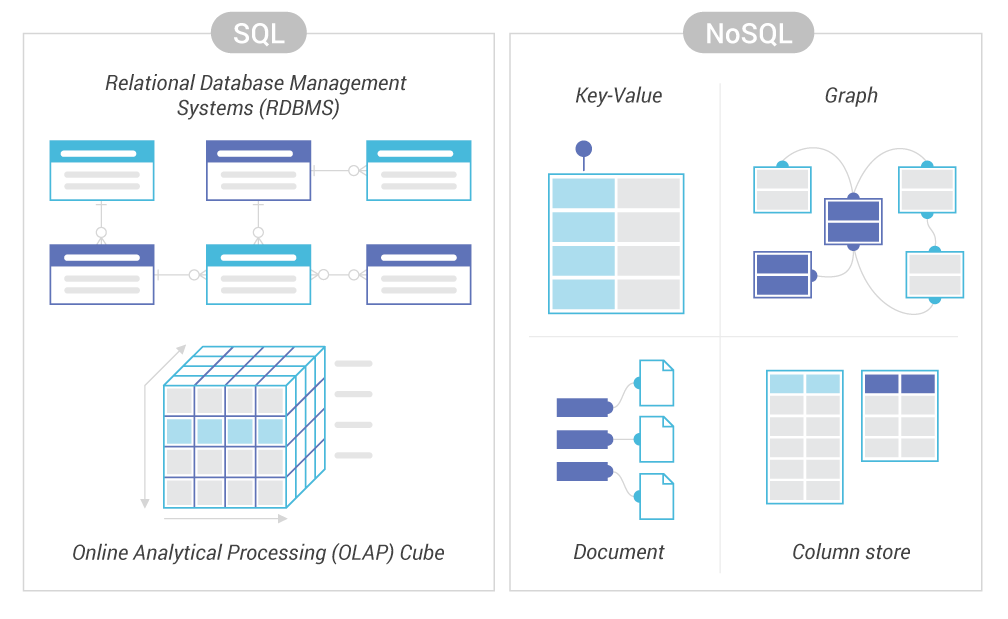
\includegraphics[width=\textwidth]{images/SQL-vs-NoSQL.png}
    \label{fig:sql_vs_nosql}
\end{figure}

\subparagraph{SQL vs NoSQL}
In Figure \ref{fig:sql_vs_nosql} you can see the abstracted way to think about these two different systems. SQL records are exactly that, a record at a point in time. If one entity encapsulates another then another table holds that information. In NoSQL, the information is abstracted to a document with key-value pairs to get specific data. These documents can make references to other documents but for time-ordering this is highly ineffective. SQL records are highly effective for logs and indexing a large amount of data based on a higher level entity such as user that has many garden beds; garden beds that have a lot of data, etc.

\subparagraph{MySQL vs PostgreSQL}
The two SQL databases widely used in industry are MySQL and PostgreSQL. MySQL is touted as ``a simple relational database [... that is] very efficient and user-friendly'' while PostgreSQL is widely used in data analytic and scientific applications because of the extensibility, scalability and object models. Immediately this seems like the better option but PostgreSQL may be harder to stand up immediately. Special consideration should be given to AWS solutions as well. 

\subparagraph{MongoDB vs DynamoDB}
MongoDB is ``a general-purpose, document-based'' database. DynamoDB is AWS' proprietary solution to NoSQL databases. DynamoDB is more difficult to work with as it is the newer service, it could also potentially be more expensive over time, however, DynamoDB has improvements over MongoDB for indexing and building out reference documents. 

\subsubsection{Proportional-integral-derivative Control}
Proportional-integral-derivative control (PID control) is a common control algorithm (espectially in industrial control systems) to allow a control loop to have reliable performance in a variety of conditions. Simply put, this algorithm allows a controller to receive an input and calculate a proportional output, accounting for error and rapid changes in the process. This algorithm may be useful to our application because it will allow the product to better control its facilities without user input.

The control function is defined in \autoref{eq:pid_controller}, where $u(t)$ is the control variable (e.g. the garden bed's water control solenoid), $K_p$, $K_i$, and $K_d$ are gain factors, and $e(t)$ (the error) is the different between a desired setpoint and measured process variable (e.g. the difference between the desired and current ounces of water dispensed).
\begin{equation}
    \label{eq:pid_controller}
    u(t) = K_pe(t) + K_i\int_{0}^{t}e(\tau) \, d\tau + K_d\frac{de(t)}{dt}
\end{equation}

\paragraph{Proportional Term} The proportional term of \autoref{eq:pid_controller} is $K_pe(t)$, hence referred to as the P-term. The P-term is proportional to the current error, and the gain $K_p$ determines the magnitude of the P-term. If the gain is too large, then the process variable will oscillate.

\paragraph{Integral Term} The integral term of \autoref{eq:pid_controller} is $K_i\int_{0}^{t}e(\tau) \, d\tau$, hence referred to as the I-term. This term accounts for previous values of $e(t)$ by taking the integral of the error, and the gain $K_i$ determines the magnitude of the I-term. The I-term aims to account for residual error in the control loop.

\paragraph{Derivative Term} The integral term of \autoref{eq:pid_controller} is $K_d\frac{de(t)}{dt}$, hence referred to as the D-term. The D-term aims to control future values of $e(t)$ by taking the derivative of the error, and the gain $K_d$ determines the magnitude of the D-term. This term acts to damp rapid changes in the control loop. Higher values of gain may make the control loop more sensitive to noise and lead to instability.

\subsubsection{Arduino Impletmentation of Microcontroller Internet Connection} Our team ultimately decided to implement a Texas Instruments microcontroller (detailed later) in the controls subsystem. This TI MCU contains an integrated network stack, and offers simple directions on connecting a compatible 2.4 GHz antenna. However, the one drawback our team did not expect was the relative abstractness, complication, and bureaucracy of creating programming with the tools required by TI. Between their proprietary distrobution of Eclipse, the libraries and SDKs required by the compiler, the configuratio of the compiler and linker, and the relative abstractness and complication of their libraries located in the SDK, the TI MCU is difficult to work with if the developer does not have pervious experience. In this section, Arduino's implementation is investigated and compared to our current TI MCU.

\paragraph{Arduino} Arduino is a microcontroller development board (integrating ATmega microcontrollers) distributor with a focus on hobbyists, especially entry-level developers. Compared to Texas Instruments, an industry-focused manufacturer, Arduino development has a very low bar to entry. Because of this, the fine granular control that may be required of an enterprise-level project is not present on Arduino boards---however, there are major advantages that make considering Arduino over TI worthwile:
\begin{itemize}
    \item Libraries are easy to implement
    \item The compiler and linker are relatively easy to configure compared to TI
    \item Large community following, support
    \item 3rd-party libraries are common and accessible
    \item Lower cost of components
    \item Easier to source components (in the year 2022)
    \item "Shields" (e.g. WiFi, GSM/GPRS, Bluetooth, GPS, motor controller, etc.) easily implementable
\end{itemize}
\paragraph{GSM/GPRS} One shield offered by Arduino is the \href{https://store.arduino.cc/products/arduino-mkr-gsm-1400}{Arduino MKR GSM 1400}, a 3G cellular network shield that enables SMS, voice, and internet connection. Arduino's library gives various "from scratch" examples and ample documentation on how to use different parts of its 1st-party \href{https://docs.arduino.cc/retired/archived-libraries/GSM}{GSM library}. For example, if one would like to connect a GSM network, it's as simple as including \texttt{GSM.h}, instantiating the \texttt{GSM} class (e.g. \texttt{GSM gsmAccess;}), and calling \texttt{begin()} (e.g. \texttt{gsmAcess.bein()}).

\paragraph{WiFi} Arduino offers shields like the \href{https://store.arduino.cc/products/arduino-mkr-wifi-1010}{Arduino MKR WiFi 1010}, as well as complete development boards like the \href{https://store.arduino.cc/products/arduino-uno-wifi-rev2}{Arduino Uno WiFi Rev2} with integrated WiFi modules. Just like the GSM library, Arduino's \href{https://www.arduino.cc/reference/en/libraries/wifi/}{WiFi library} is very easy to implement and use, and its documentation is wholly informative with class and function definitions and plenty of examples. For example, all one need do to connect to a network is detailed in the example in \autoref{fig:arduino_wifi_example}.

\begin{figure}[hbtp]
    \caption{Arduino WiFi code example}
    %\centering
    \label{fig:arduino_wifi_example}
    \begin{lstlisting}[language=c,frame=none,numbers=left,numbersep=-10pt,numberstyle=\tiny,basicstyle=\footnotesize\ttfamily]
        #include <WiFi.h>

        char ssid[] = "exampleNetwork";
        void setup() {
            while (status != WL_CONNECTED) {
                // Attempt to connect to SSID
                status = WiFi.begin(ssid);

                // Wait 10 seconds
                delay(10000);
            }

            // Once you reach here, you're connected
    \end{lstlisting}
\end{figure}

The user can go on to perform many different functions, with the limitation that they are either TCP or UDP bytestreams. This differs greatly from the TI CC3200's multifunctionality of being able to perform HTTP requests, Websockets, and many more on top of being able to take advantage of TCP and UDP bytestreams.